%%%
% credits: https://tex.stackexchange.com/questions/431093/3d-cartesian-coordinate-system


\scalebox{0.35}{ %%% scalebox
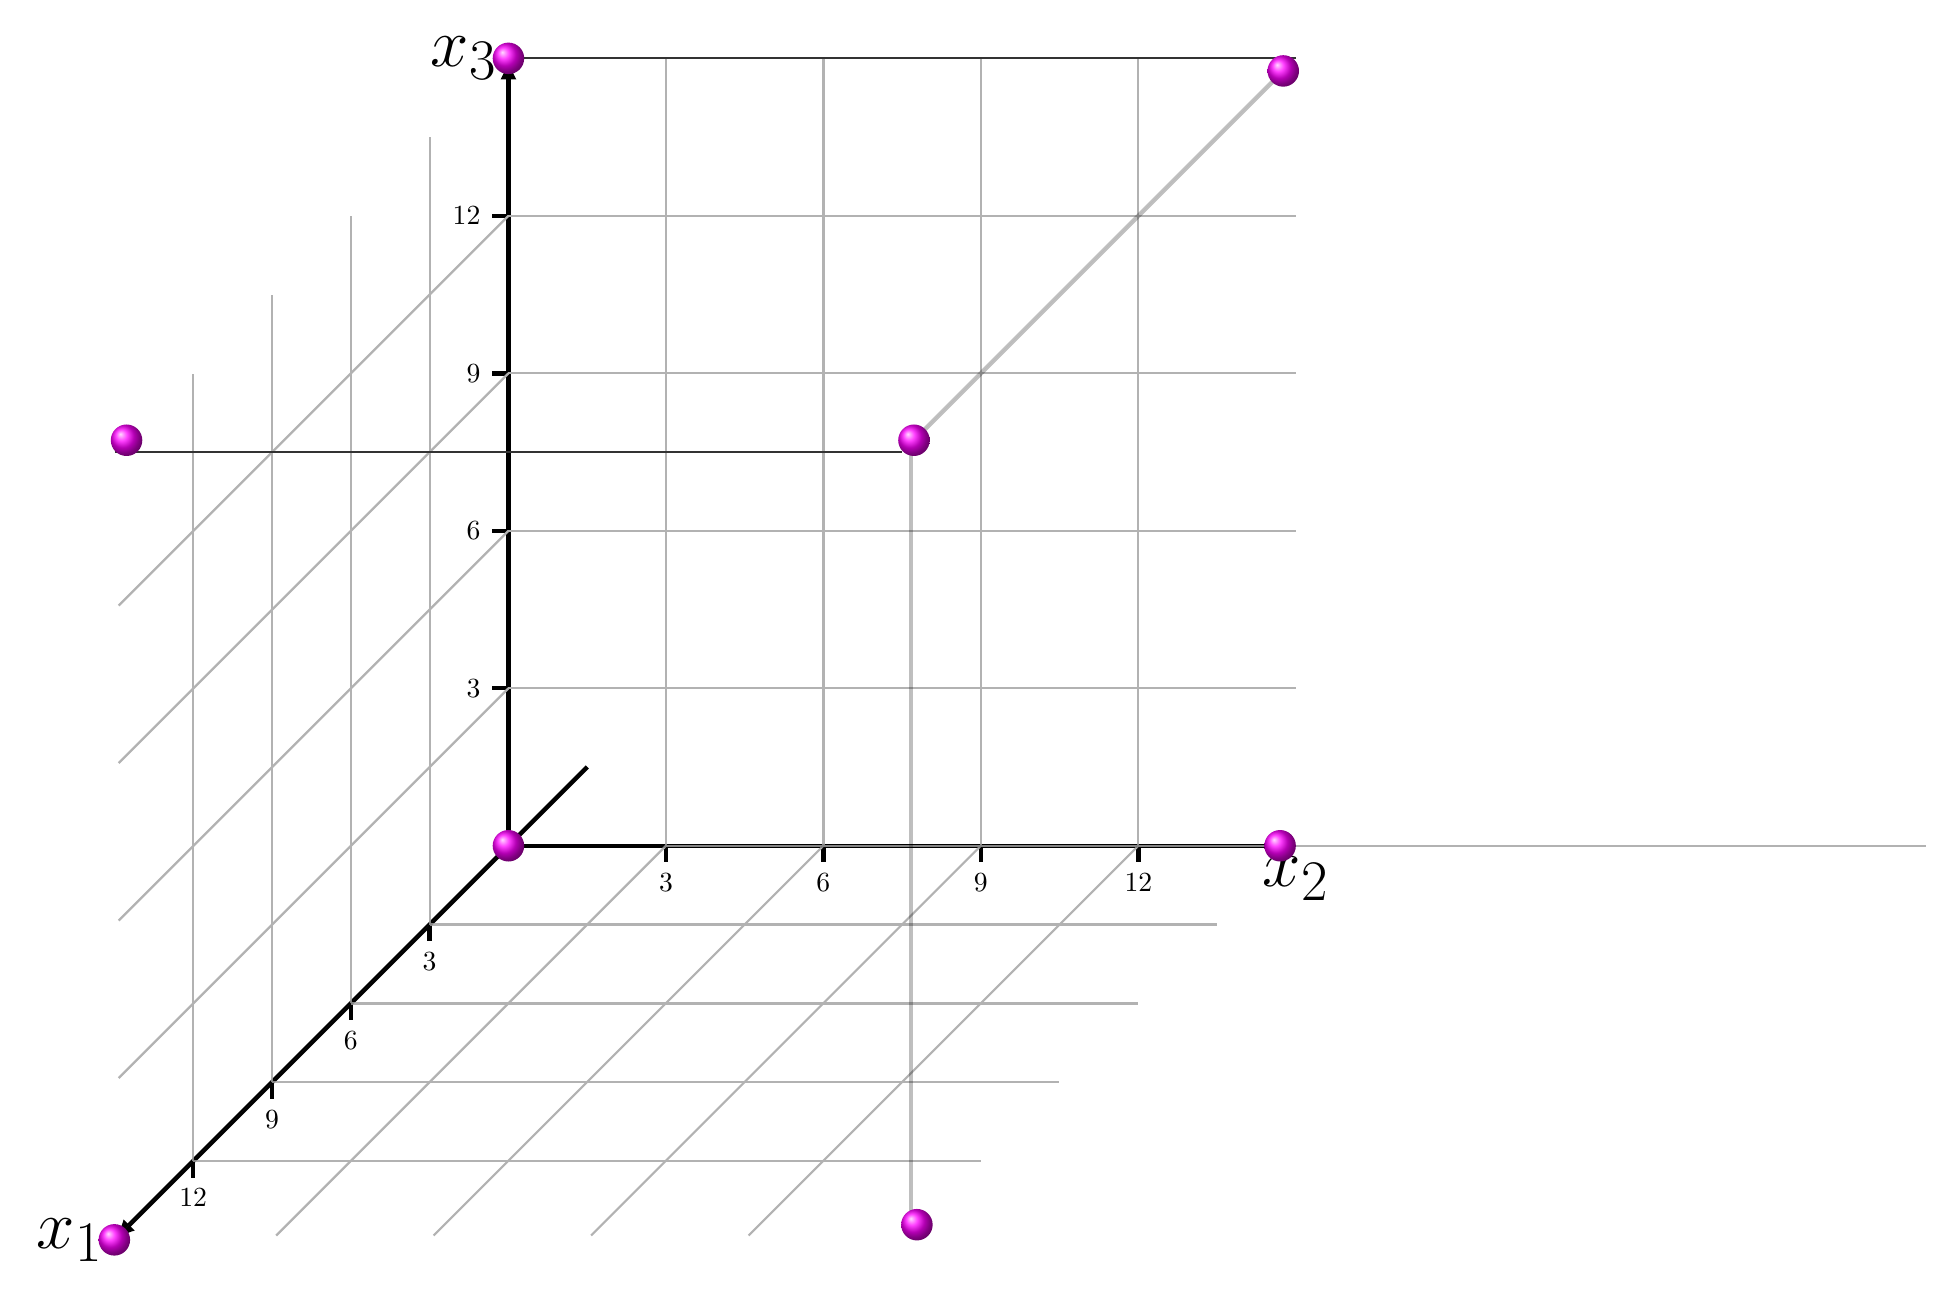
\begin{tikzpicture}
    %\draw[gray!60!white, thick] (-4.99,-4.99) grid (9.99,9.99);
    \draw[->, >=latex, ultra thick] (0,0,-2.6) -- (0,0,13) node[left]{\Huge{$x_1$}};
    \draw[->, >=latex, ultra thick] (0,0,0) -- (10,0,0) node[below]{\Huge{$x_2$}};
    \draw[->, >=latex, ultra thick] (0,0,0) -- (0,10,0) node[left]{\Huge{$x_3$}};
    % grid lines and axis ticks
    \foreach \z/\zc in {2.6/3,5.2/6,7.8/9,10.4/12}{
        \draw[shift={(0,0,\z)}, ultra thick] (0pt,0pt,0pt) -- (0pt,-0.21pt,0pt)node[below]{\zc};
        \draw[gray!60!white, thick](0,0,\z)--++(0:10);
        \draw[gray!60!white, thick](0,0,\z)--++(90:10);
    }
    \foreach \x/\xc in {2/3,4/6,6/9,8/12}{
        \draw[shift={(\x,0)}, ultra thick] (0pt,0pt) -- (0pt,-6pt)node[below]{\xc};
        \draw[gray!60!white, thick](\x,0)--++(0:10);
        \draw[gray!60!white, thick](\x,0)--++(90:10);
        \draw[gray!60!white, thick](\x,0)--++(-135:7);
    }
    \foreach \y/\yc in {2/3,4/6,6/9,8/12}{
        \draw[shift={(0,\y)}, ultra thick] (0pt,0pt) -- (-6pt,0pt)node[left]{\yc};
        \draw[gray!60!white, thick](0,\y)--++(0:10);
        \draw[gray!60!white, thick](0,\y)--++(-135:7);
    }
    %aux grid lines
    \draw[black!80!white, thick](0,10)--++(0:10);
    \draw[black!80!white, thick](-5,5)--++(0:10);
    
    % 3 planes
    \draw[fill=black!30, ultra thick, nearly transparent] (0,0,0) -- (0,0,12.7);
    \draw[fill=black!30, ultra thick, nearly transparent] (0,0,0) -- (9.9,0,0);
    \draw[fill=black!30, ultra thick, nearly transparent] (9.9,9.9,0) -- (9.9,9.9,12);
    \draw[fill=black!30, ultra thick, nearly transparent] (10,0,12.7) -- (10,10,12.7);
    % points
    \shade[ball color=magenta] (16,16,16) circle (0.2);
    \shade[ball color=magenta] (9.8,0,0) circle (0.2);
    \shade[ball color=magenta] (0,0,13) circle (0.2);
    \shade[ball color=magenta] (9,9,10) circle (0.2);
    \shade[ball color=magenta] (0,10,0) circle (0.2);
    \shade[ball color=magenta] (-1,9,10) circle (0.2);
    \shade[ball color=magenta] (10,0,12.5) circle (0.2);
    \shade[ball color=magenta] (0,0,0) circle (0.2);
\end{tikzpicture}
} % scale
